\documentclass[12pt,a4paper,openany]{book}
\usepackage{lmodern}
\usepackage[svgnames]{xcolor} % Required to specify font color
\input{/home/aroquemaurel/cours/includesLaTeX/couleurs.tex}

\usepackage[utf8]{inputenc} \usepackage[T1]{fontenc}
\usepackage[final]{pdfpages} 

\usepackage[francais]{babel}
\usepackage[top=1.7cm, bottom=1.7cm, left=1.7cm, right=1.7cm]{geometry}
\usepackage{verbatim}
\usepackage[urlbordercolor={1 1 1}, linkbordercolor={1 1 1}, linkcolor=vert1, urlcolor=bleu, colorlinks=true]{hyperref}
\usepackage{tikz} %Vectoriel
\usepackage{listings}
\usepackage{fancyhdr}
\usepackage{multido}
\usepackage{float}
\usepackage{amssymb}
\usepackage{longtable}
\usepackage{wrapfig}

\newcommand{\titre}{Projet de programmation}
\newcommand{\subtitle}{Partie Java}
\newcommand{\auteur}{Dario \bsc{Olibet} et Antoine de \bsc{Roquemaurel}}
\newcommand{\formation}{L3 Informatique}
\newcommand{\semestre}{5}
\newcommand{\annee}{2014}
\newcommand{\prof}{}


\newcommand{\pole}{}
\newcommand{\sigle}{pf1}


\input{/home/aroquemaurel/cours/includesLaTeX/listings.tex}
\date{\today}

\makeindex
\lfoot{Université Toulouse III -- Paul Sabatier}
\rfoot{}
%\rfoot{}
\cfoot{}
\makeglossary
\makeatletter
\def\clap#1{\hbox to 0pt{\hss #1\hss}}%
\def\ligne#1{%
\hbox to \hsize{%
\vbox{\centering #1}}}%
\def\haut#1#2#3{%
\hbox to \hsize{%
\rlap{\vtop{\raggedright #1}}%
\hss
\clap{\vtop{\centering #2}}%
\hss
\llap{\vtop{\raggedleft #3}}}}%
\def\bas#1#2#3{%
\hbox to \hsize{%
\rlap{\vbox{\raggedright #1}}%
\hss \clap{\vbox{\centering #2}}%
\hss
\llap{\vbox{\raggedleft #3}}}}%
\def\maketitle{%
\thispagestyle{empty}\vbox to \vsize{%
\haut{}{\@blurb}{}

\vfill
\vspace{1cm}
\begin{flushleft}
\usefont{OT1}{ptm}{m}{n}
\huge \@title
\end{flushleft}
\par
\hrule height 4pt
\par
\begin{flushright}
\usefont{OT1}{phv}{m}{n}
\Large \@author
\par
\end{flushright}
\vspace{1cm}
\vfill
\vfill
\bas{}{\@location, le \@date}{}
}%
\cleardoublepage
}
\def\date#1{\def\@date{#1}}
\def\author#1{\def\@author{#1}}
\def\title#1{\def\@title{#1}}
\def\location#1{\def\@location{#1}}
\def\blurb#1{\def\@blurb{#1}}
\date{\today}
\author{}
\title{}
\location{Amiens}\blurb{}
\makeatother
\title{\titre}
\author{Partie Java}

\location{Toulouse}
\blurb{%
Université Toulouse III -- Paul sabatier\\
L3 Informatique\\
\vspace{30px}
\begin{flushleft}Antoine de \bsc{Roquemaurel} \\ 
	Dario \bsc{Olibet} \\
 Groupe 1.1\end{flushleft}
}%



%\title{Cours \\ \titre}
%\date{\today\\ Semestre \semestre}

%\lhead{Cours: \titre}
%\chead{}
%\rhead{\thepage}

%\lfoot{Université Paul Sabatier Toulouse III}
%\cfoot{\thepage}
%\rfoot{\sigle\semestre}

\pagestyle{fancy}
\renewcommand{\chaptermark}[1]{\markboth{\bsc{\chaptername~\thechapter{} :} #1}{}}
\renewcommand{\sectionmark}[1]{\markright{\thesection{ #1}}}
\renewcommand{\headrulewidth}{0.3pt}
\renewcommand{\footrulewidth}{0.3pt}

\fancyhf{}
\fancyhead[LE]{\leftmark}
\fancyhead[RO]{\rightmark}
\fancyfoot[LE,RO]{--~\thepage~--}
\fancyfoot[LO]{\titre{}}
\fancyfoot[RE]{Antoine de \bsc{Roquemaurel} -- Dario \bsc{Olibet}}

%% Cas des premières pages de chapitre
\fancypagestyle{plain}{%
	\fancyhf{}%
	\fancyfoot[L]{\titre{}}
	\fancyfoot[R]{--~\thepage~--}
	\renewcommand{\headrulewidth}{0pt}
	\renewcommand{\footrulewidth}{0.3pt}
}
\makeatletter
\renewcommand*{\lstlistlistingname}{Liste des codes sources}
\renewcommand\listoffigures{%
    \chapter{\listfigurename}%
      \@mkboth{\MakeUppercase\listfigurename}%
              {\MakeUppercase\listfigurename}%
       \@starttoc{lof}%
    }
    \renewcommand\listoftables{%
    \chapter{\listtablename}%
    \@mkboth{\MakeUppercase{\listtablename}}%
            {\MakeUppercase{\listtablename}}%
    \@starttoc{lot}
    }

    \renewcommand\lstlistoflistings{%
    \begingroup
    \chapter{\lstlistlistingname}%
    \parskip\z@\parindent\z@\parfillskip \z@ \@plus 1fil%
    \@starttoc{lol}%
    \endgroup
    }
	\makeatother

\input{/home/aroquemaurel/cours/includesLaTeX/remarquesExempleAttention.tex}
\input{/home/aroquemaurel/cours/includesLaTeX/polices.tex}
\input{/home/aroquemaurel/cours/includesLaTeX/affichageChapitre.tex}
\let\pagebreakORIG\pagebreak
\let\clearpageORIG\clearpage
\let\cleardoublepageORIG\cleardoublepage

\ifx \removepagebreak \undefined
\newcommand{\removepagebreak}{\renewcommand{\pagebreak}{}\renewcommand{\clearpage}{}\renewcommand{\cleardoublepage}{}}
\fi

\ifx \restorepagebreak \undefined
\newcommand{\restorepagebreak}{\renewcommand{\pagebreak}{\pagebreakORIG}\renewcommand{\clearpage}{\clearpageORIG}\renewcommand{\cleardoublepage}{\cleardoublepageORIG}}

\fi
\newcommand{\pfp}{\texttt{pfp}}

%\newcommand{\ifp}{\texttt{if}}
%\newcommand{\elsep}{\texttt{else}}

\input{/home/aroquemaurel/cours/includesLaTeX/couvertureProjet.tex}
\makeatother
\includeonly {
}
\newcommand{\bootstrap}{\textit{bootstrap}}
\begin{document}
	\thispagestyle{empty} % Removes page numbers
	\titleBC 
	\setcounter{tocdepth}{2}
	\setcounter{secnumdepth}{3}
	\newpage
	\chapter*{Avant-propos}
	Ce dossier comporte l'organisation et les étapes de développement d'un projet d'Arènes en Java. 

	Il à été conçut par Dario \bsc{Olibet} et Antoine de \bsc{Roquemaurel} dans le cadre du module \textit{Projet de programmation} de la L3
	Informatique de l'université Toulouse III -- Paul Sabatier.\\~

	\large{\sectionfont Contenu de l'archive du projet}\\
	\normalsize
	L'archive que vous avez reçus était organisée comme ceci: 
	\begin{description}
		\item[\texttt{rapport.pdf}] Le présent rapport que vous êtes en train de lire
		\item[\texttt{v1Arene/}] Contient le dossier avec la première version de l'application : notre propre arènes avec les règles que nous avons implémentées. 
		\item[\texttt{v1Arene/doc/}] Contient la documentation de la première version du projet. Celle-ci à été générée à l'aide de \textit{Doxygen}, elle
			est disponible en HTML ou en PDF (générée avec \LaTeX).

			L'utilisation de \textit{Doxygen} contrairement à \textit{Javadoc} permet d'avoir une génération en PDF, mais également d'avoir l'apparition des diagrammes de
			classes ce qui facilite la compréhension du problème.
		\item[\texttt{V2Commun/}] Contient le dossier avec la version contenant notre stratégie pour l'arène commune distante. Les seuls fichiers que nous avons
			modifiés par rapport à la version de base sont les classes \texttt{Console}, \texttt{TestConsole} et \texttt{TestConsoleObjet}.
	\end{description}

	Le projet à été développé en Java6.

	\vfill
	\footnotesize Rédigé le \today{} par Dario \bsc{Olibet} et Antoine de \bsc{Roquemaurel}.
	\tableofcontents
	\chapter{Organisation du travail d'équipe}
	Pour ce projet, nous étions deux à travailler dessus, ainsi nous avons utilisé plusieurs techniques afin de se coordonner et de limiter les problèmes. Ceci
	n'est pas notre premier projet ensemble, notre travail en fut simplifié.
	\section{Un outil de gestion de projet : Redmine}
	Pour le projet, nous avons utiliser \textit{Redmine}, une plateforme web de gestion de projet. Elle nous a permis de simplifier le travail,
	à ne rien oublier et à nous répartir le travail.

	En effet, nous pouvons créer des tâches, signaler qu'elles sont en cours/terminés/en tests, leur donner des dates limites, les affecter à une personne etc\ldots
	Ainsi lorsque l'un de nous commençait une tâche, il le signalait sur le \textit{redmine}, ce qui permettait de tenir au courant son binôme de ses actions et
	de l'avancée du projet.

	Nous nous sommes également servis du wiki que possède Redmine, ainsi nous avons pu y déposer des conventions d'écritures afin d'avoir un code qui soit
	cohérent, simple à relire et homogène. Les conventions sont disponibles en annexe \ref{conventions} page \pageref{conventions}.
	\begin{figure}[H]
		\centering
		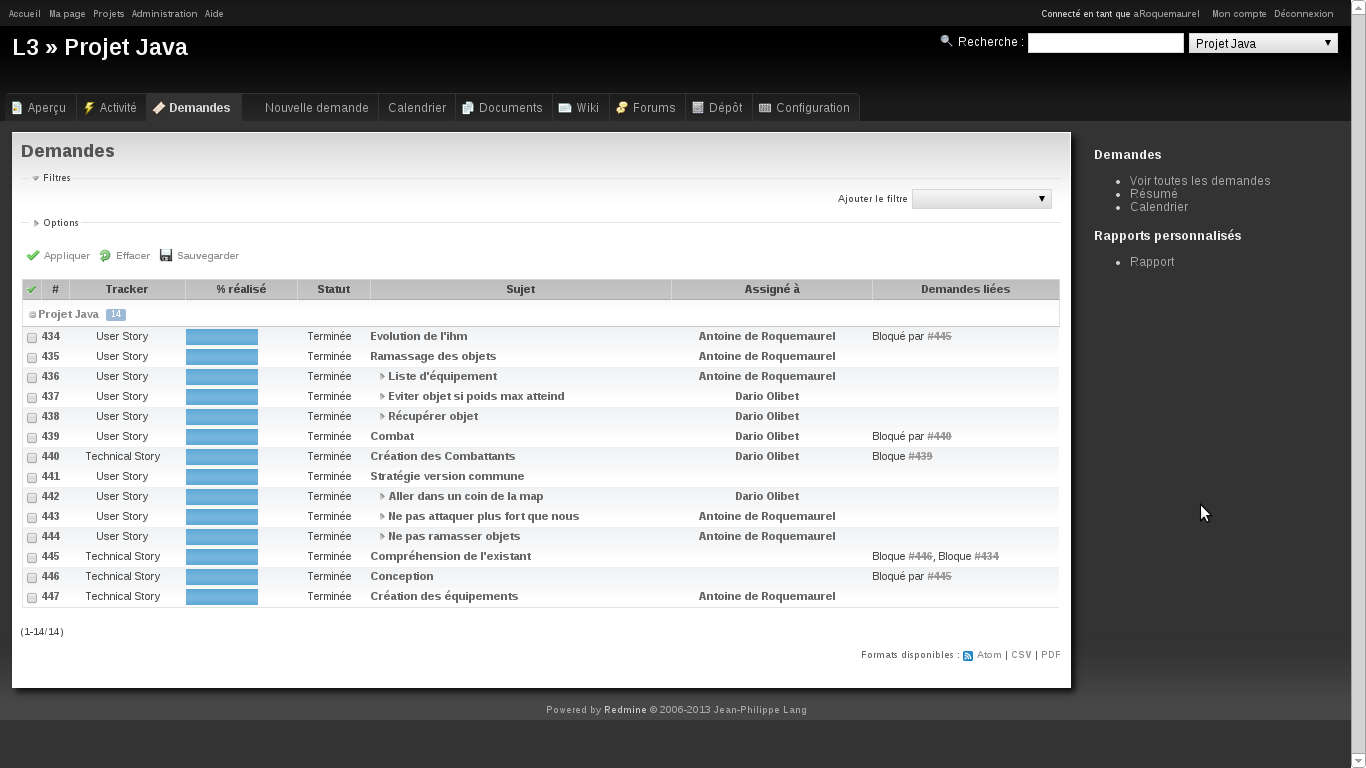
\includegraphics[width=18cm]{screens/redmine.png}
		\caption{Liste des tâches sous Redmine}
	\end{figure}

	\section{Un logiciel de versionnement : Git}
	Afin de limiter les problèmes du travail collaboratif, nous avons utilisé un logiciel de versionnement Git. Il a deux intérêt, tout d'abord, nous pouvons
	travailler à deux en parallèle sur le projet sans se soucier de fusionner notre travail\footnote{À condition de ne pas travailler sur deux lignes de code
	identiques}.

	D'autre part, tous les logs étant enregistrés, nous pouvons savoir qui à fait quoi et quel jour, cela permet de voir également l'avancée du projet. 

	Enfin, toutes les modification sont stockées sur le serveur, ainsi en cas de problème, il est très facile de revenir à la version précédente ou même de
	comparer deux versions afin de voir les changements et de comprendre rapidement pourquoi une fonctionnalité à régressé. 

	Nous avons aussi pu nous en servir afin d'effectuer des branches de tests.

	\chapter{Première version : local}
	\section{Règles du jeu}
	Nous avons décidés d'implanter des règles basé sur d'une part les combattants et d'autre part les équipements. Afin de gagner une partie le combattant doit
	être le dernier en vie dans l'arène.
	\subsection{Combattant}
	Chaque personnage dispose de caractéristiques, ces caractéristiques doivent respecter une règle d'équilibre. Si cette règle n'est pas respectée, le joueur
	n'est pas accepté sur le serveur : $\frac{vie}{10} + Attaque + Défense + Vitesse = 10$.
	\subsection{Caractéristiques}
	\begin{description}
		\item[Nombre de point de vie] Chaque personnage dispose d’un certain nombre de pv\footnote{Point de vie}.
		\item[Attaque/Force] La force d'un personnage 
		\item[Vitesse/esquive] Chance pour un personnage d’éviter une attaque.
		\item[Nombre d'objets] Nombre d’objets qu'un personnage peut porter.
	\end{description}

Le nombre d'objets qu'un personnage peut porter est choisi arbitrairement et compris entre 1 et 5 et ne rentre pas dans la règle d'équilibre.

	 \begin{table}[H]
		 \centering
		 \normalsize
	 \begin{tabular}{cc|cccccp{5.0cm}}
			&&Vie& Attaque & Défense & Vitesse & Nb objet&Description\\
			\hline
			\textbf{Capitaine} & Luffy & 30 & 3 & 2 & 2 & 3& \footnotesize Équilibré\\
			\hline
			\textbf{Barde} & Brook & 10 & 2 & 3 & 4 & 2& \footnotesize Peu résistant mais ayant une bonne défense et une bonne fuite\\
			\hline
			\textbf{Spadassin} & Zorro & 20 & 4 & 1& 3&1& \footnotesize Préfère un combat rapide tout en essayant d'éviter un maximum d'attaques\\
			\hline
			\textbf{Cyborg} & Franky & 20 & 3 & 4 & 1& 4 & \footnotesize Défensif et fort, mais très lent\\
			\hline
			\textbf{Mascotte} & Chopper&20&1&3&4&5& \footnotesize Bonne défense et bonne fuite. \\
			\hline
		\end{tabular}
		\caption{Les différentes classes de personnage créées}
	\end{table}

\subsection{Combat}
Lorsqu'un combat à lieux, deux règles sont mises en place.

La première est basée sur l'esquive: la vitesse multipliée par 10 est le pourcentage de chances d’esquiver une attaque, lorsqu'une attaque est esquivée, aucun
dégât n'est subi. 

La deuxième est basée sur le ratio entre l'attaque et la défense, si l'attaque de l'attaquant est supérieure à la défense du défenseur nous avons : $attaque
- défense =  dégâts$ qui sont infligés au défenseur. Dans le cas où son attaque est inférieure à la défense, un seul point de dégât est causé.

	\subsection{Équipements}
	 Un équipement peut donner un ou plusieurs bonus d'attaque, défense et vitesse. Tout équipement à une durée de vie qui correspond aux nombre de tours qu'un
	 personnage l'utilise, ce nombre de tours est choisis arbitrairement entre 1 et 5\footnote{Nous avons essayer d'avoir une certaine logique, en fonction du
	 type de l'équipement. Par exemple un plastron aura une plus grande durée qu'une canne}.

	 Nos équipements sont tous équilibrés. Ils donnent un bonus total de 2 et un malus total de 1, donc $bonusAttaque+bonusDefense+bonusVitesse = 1$.
	 Chaque personnage peut récupérer n'importe quel équipement mais chacun d’eux à une préférence selon sa classe afin d'être le plus équilibré possible.

	 \begin{table}[H]
		 \centering
		 \normalsize
	 \begin{tabular}{cc|ccccp{5.0cm}}
			&& Attaque & Défense & Vitesse & Durée&Description\\
			\hline
			{Chapeau de paille} & Luffy & 1 & -1 & 1 & 2 & \footnotesize \\
			\hline
			{Canne} & Brook & 2 & -1 & 0 & 1 & \footnotesize \\
			\hline
			{Sabre} & Zorro & 2 & 0 & -1& 4& \footnotesize \\
			\hline
			{Plastron} & Franky & 0 & 2 & -1 & 5 & \footnotesize \\
			\hline
			{Bottes} & Chopper&-1&0&2&3& \footnotesize \\
			\hline
		\end{tabular}
		\caption{Les différents équipements créés}
	\end{table}

	\section{Conception}
		Afin de concevoir au mieux l'application, nous avons tout d'abord étudié le code source existant. Une fois que nous avons compris son fonctionnement,
		nous avons définis nos équipements et nos personnes en fonction d'un \texttt{Element}.

		Ci-dessous le diagramme de classe : 

		\begin{figure}[H]
			\centering
			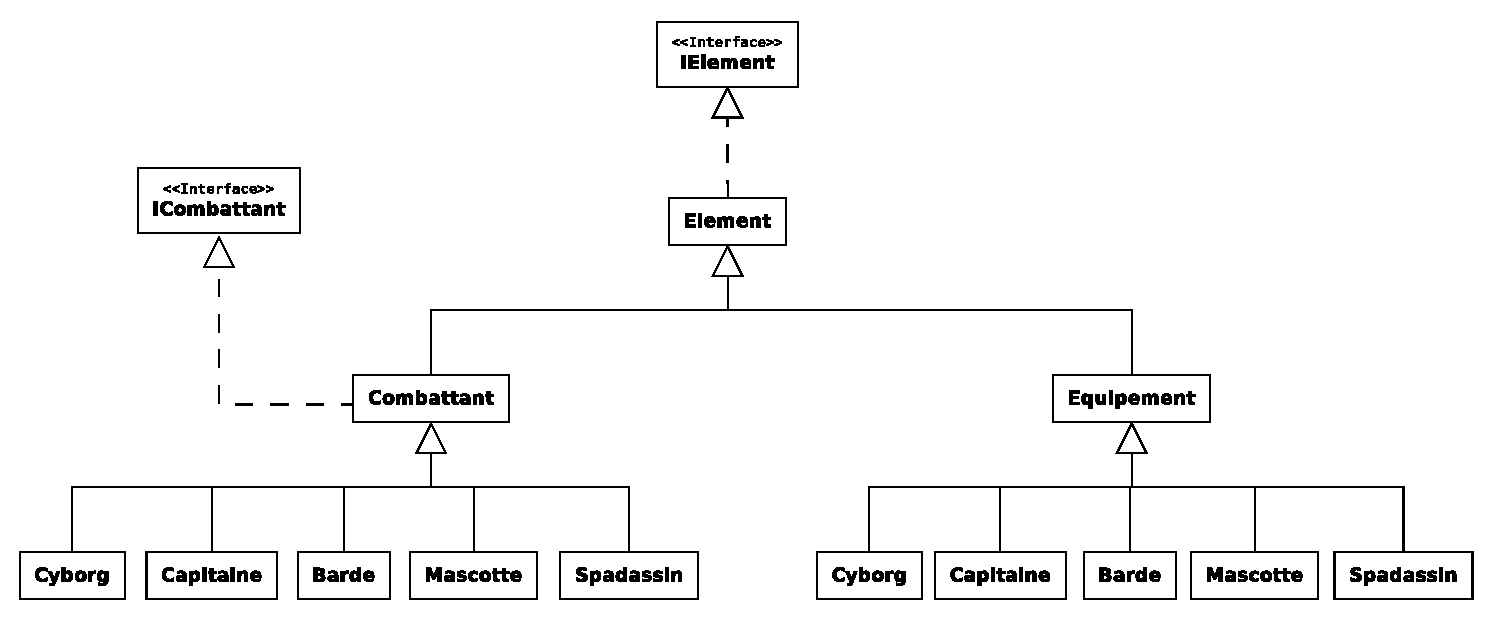
\includegraphics[width=14.5cm]{Diagramme1.eps}
			\caption{Diagramme de classe des \texttt{Element}}
		\end{figure}

		Une fois ces classes créés, il fallait implémenter les règles du jeu, pour cela nous avons modifiés le serveur afin que les personnages puissent : 
		\begin{itemize}
			\item Ramasser des objets, s'il en a la possibilité (vérification du poids) Classe \texttt{Arene}
			\item Implémentation des duels : Classe \texttt{DuelBasic}
			\item Vérification du respect de la règle d'équilibre : Classe \texttt{Arene}
			\item Ajout du port d'objets dans le calculs des statistiques : Classe \texttt{ListeEquipements}.
		\end{itemize}

		Nous avons également modifié un peu l'IHM afin de distinguer la différence entre un objet et un personnage : les objets sont représenté par un carré
		alors que les combattants par des ronds.

		L'architecture de notre jeu est donc assez classique, mis-à-part la gestion de la possession des équipements. Nous avons choisis de créer une nouvelle
		classe \texttt{ListeEquipement} héritant de \texttt{ArrayList}, ce qui nous a permis de simplifier au maximum le reste de notre code. Une simple
		surcharge de la méthode \texttt{add} nous a permis d'ajouter un équipement uniquement si le nombre d'objets maximum n'est pas atteint. La souplesse des
		\texttt{ArrayList} nous a également permis de parcourir très facilement la liste d'équipement à l'aide des \texttt{Iterateur}.

	\chapter{Seconde Version : commun}
	\section{Stratégie}
Notre personnage, Franky a pour caractéristiques une attaque de 65 et une défense de 35. Il ne possède donc aucune esquive et aucune possibilité d’avoir un
équipement. 

Nous avons adapté notre objet ainsi que notre stratégie par rapport à ces caractéristiques. L'objet est une bombe, ayant un poids léger pour
contrer les personnages ne prenant aucun équipement faisant un poids de 0. Ses bonus/malus sont : 2 de force, 0 de défense, 0 d'esquive et un malus de
100 en vie. Ayant un bonus de 2 en force son poids était donc de $2 \times \frac{3}{4} = 1.5$ arrondi à 1. Nous nous débarrassons ainsi d’un possible ennemi, qui, après une certaine
durée, pourrait avoir des statistiques pouvant nous battre. 

La stratégie de notre combattant est, dans une première partie, de se diriger dans le coin le plus
proche de l'arène et rester dans un coin de $30\times 30$ pendant 2 minutes. Une fois que ce temps est écoulé notre personnage décide d'errer dans la totalité de
l'arène en cherchant le combat, maintenant que les personnes se sont entretuées. Si il voit un adversaire ayant plus de vie que lui, il fuit en espérant que
quelqu'un le rendra plus faible pour pouvoir gagner plus tard.

\section{Implémentation}
Afin d'implémenter cette stratégie nous avons utilisé la méthode \texttt{run}. Pour la première version, nous n'avions pas effectué de stratégie et n'avions pas
cherché le moyen de contrôler le déplacement de notre personnage, ainsi une nouvelle étude du fonctionnement de \texttt{Console} nous a permis de trouver les
solutions à nos problèmes.

Nous avons donc créé un attribut permettant de compter le nombre d'actions écoulés, c'est-à-dire le nombre de fois ou \texttt{run} est lancé. C'est comme ceci
que nous avons pus dès le premier lancement du run choisir un endroit ou aller dans la map, et n'y rester qu'un certain temps.

\chapter{Les difficultés rencontrés}
		Notre difficulté principale fut la compréhension du système de \texttt{Remote}. En effet une \texttt{Arene} ne possédait qu'un
		entier comme guise de référence, la question étant comment pouvoir récupérer un \texttt{Element}, ou même mieux un \texttt{Combattant} à partir de cet
		entier. C'est en cherchant dans le projet que nous avons trouvé la solution : La récupération de la \texttt{Remote}, puis le cast vers une \texttt{Console}, récupération d'un
		\texttt{Element} avec la fonction \texttt{getElement} pour finalement caster de nouveau si le besoin s'en faisant sentir.

		Cependant, la javadoc du système étant assez complète, nous avons pu comprendre le fonctionnement de l'architecture et ainsi effectuer nos propres
		modifications.	

\appendix
\newpage
\removepagebreak
	\chapter{Liste des tâches}
	\begin{figure}[H]
		\centering
		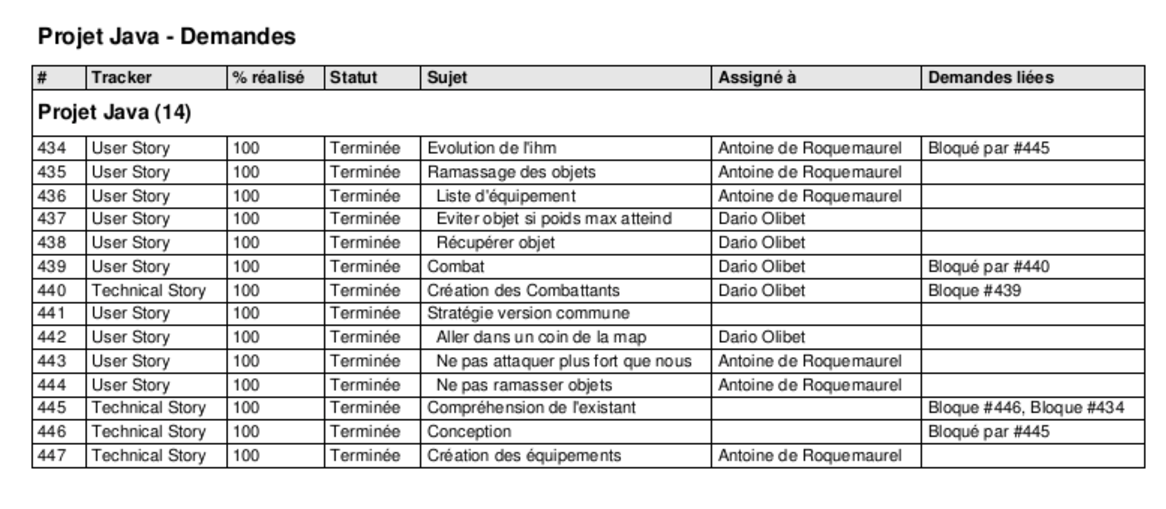
\includegraphics[width=14cm]{tachesRedmine.pdf}
		\caption{Liste des tâches Redmine}
	\end{figure}
	\vfill
	\label{conventions}
	\chapter{Conventions d'écritures}
	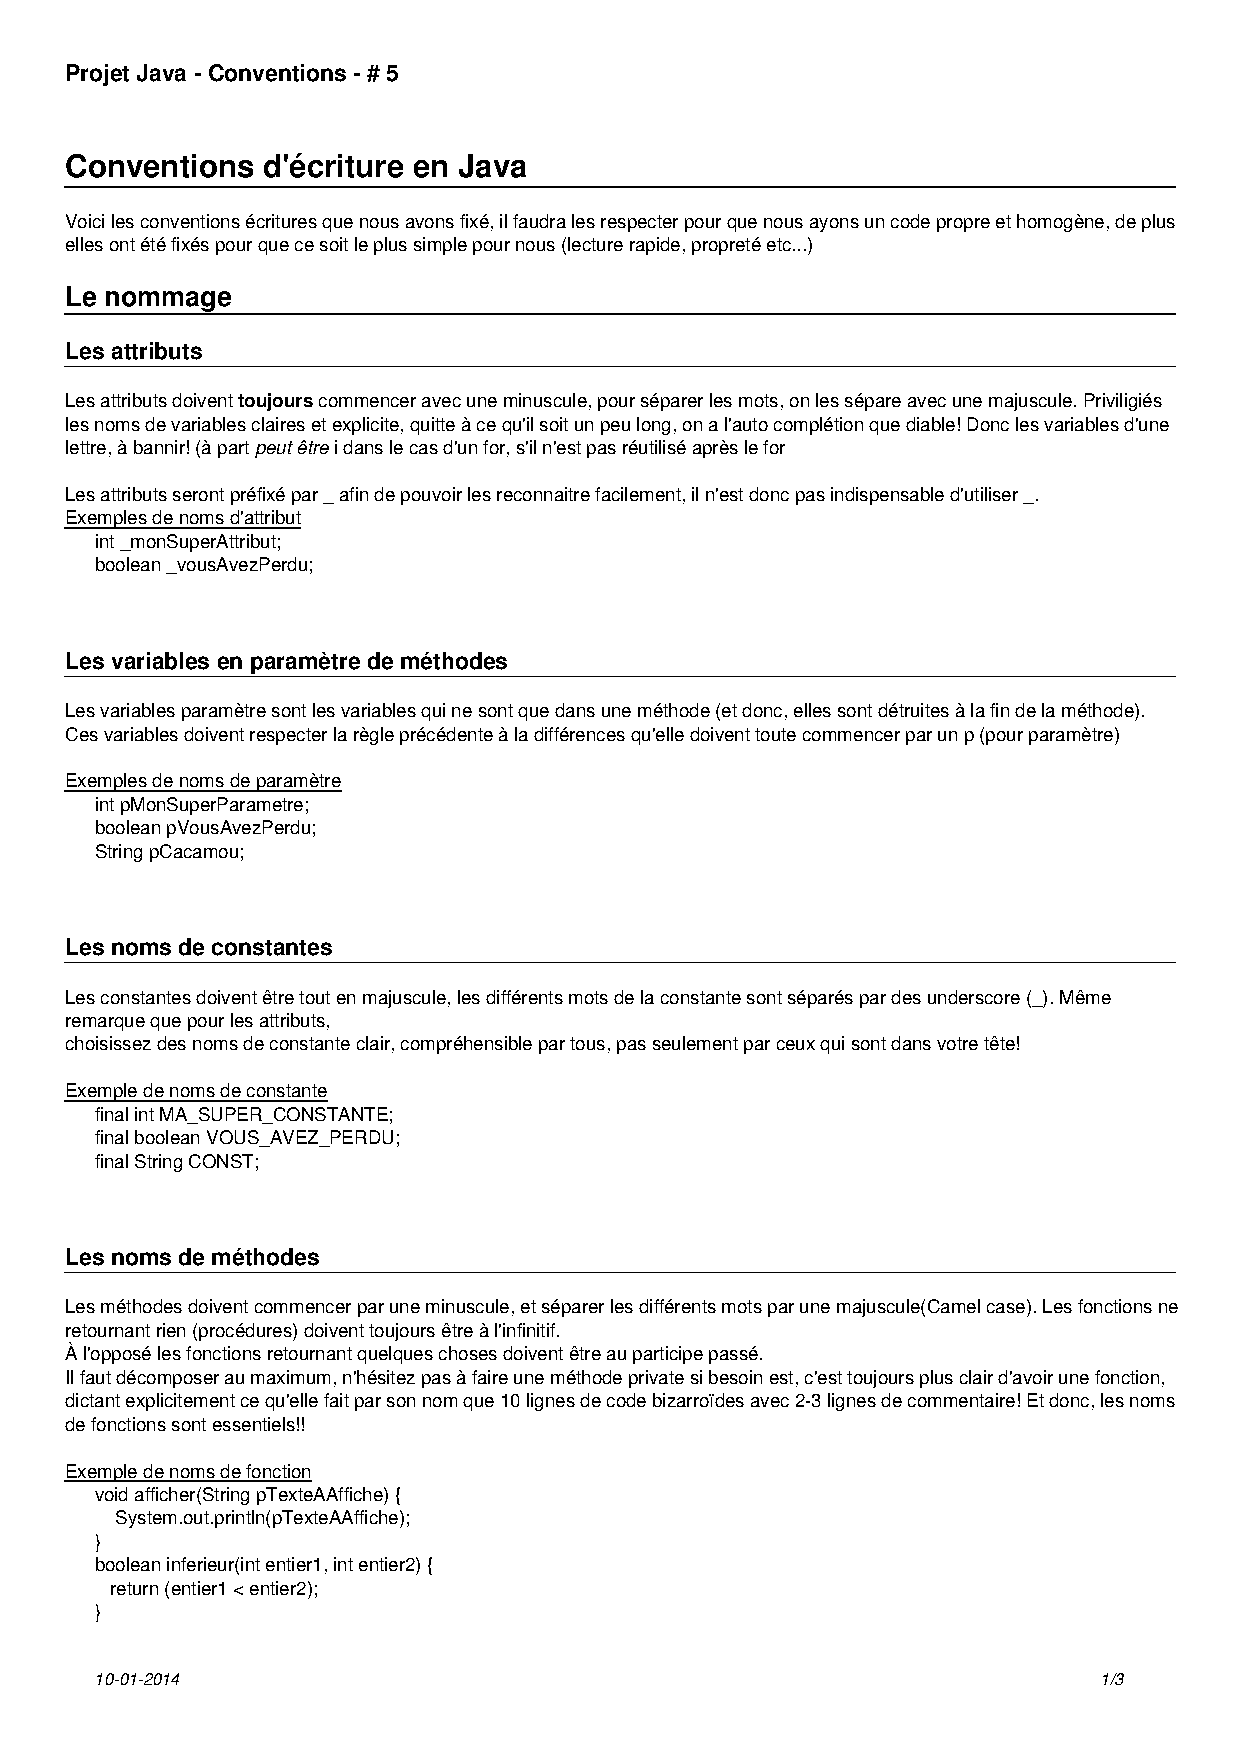
\includepdf[page=1-]{Conventions.pdf}
\listoffigures
	\vfill
	\vfill
%\lstlistoflistings
\listoftables
	\vfill
	\restorepagebreak
	
\end{document}

